\documentclass[a4paper, 12pt]{article}

\usepackage[top=2cm, bottom=2cm, left=2.5cm, right=2.5cm]{geometry}
\usepackage[utf8]{inputenc}
\usepackage{array}
\usepackage{graphicx}

\graphicspath{{img/}}

\begin{document}
\begin{flushleft}\includegraphics{logo}\\
\textbf{UNIVERSIDADE ESTADUAL DE PONTA GROSSA} \\
SISTEMA UNIVERSIDADE ABERTA DO BRASIL - UAB \\
\underline{Licenciatura em Matemática | Polo UAB em Jacarezinho}\end{flushleft} 
\textbf{ALUNO:} Ricardo Medeiros da Costa Junior   \textbf{RA:} 151774301 \\
\textbf{DISCIPLINA:} Probabilidade e Estatística 1 \\
\textbf{ATIVIDADE:} Unidade 1 - Tarefa 1 \\ 
\textbf{TUTOR(A):} Adilane de Assis Ferreira \\
\textbf{PERÍODO:} Quarto \\\\
\begin{enumerate}
\item Considere os dados obtidos pelas medidas das alturas de 100 indivíduos (dadas em cm):\\\\
  151-152-154-155-158-159-159-160-161-161 \\
  161-162-163-163-163-164-165-165-165-166 \\
  166-166-166-167-167-167-167-167-168-168 \\
  168-168-168-168-168-168-168-168-169-169 \\
  169-169-169-169-169-170-170-170-170-170 \\
  170-170-171-171-171-171-172-172-172-173 \\
  173-173-174-174-174-175-175-175-175-176 \\
  176-176-176-177-177-177-177-178-178-178 \\
  179-179-180-180-180-180-181-181-181-182 \\
  182-182-183-184-185-186-187-188-190-190 \\\\

  Construa a distrubuição de frequência:
  \begin{tabular}{c | c }
    Altura & Número de pessoas com essa altura \\
    \hline
    151 & 1 \\
    152 & 1 \\
    154 & 1 \\
    155 & 1 \\
    158 & 1 \\
    159 & 2 \\
    160 & 1 \\
    161 & 3 \\
    162 & 1 \\
    163 & 3 \\
    164 & 1 \\
    165 & 3 \\
    166 & 4 \\
    167 & 5 \\
    168 & 10 \\
    169 & 7 \\
    170 & 7 \\
    171 & 4 \\
    172 & 3 \\
    173 & 3 \\
    174 & 3 \\
    175 & 4 \\
    176 & 4 \\
    177 & 4 \\
    178 & 3 \\
    179 & 2 \\
    180 & 4 \\
    181 & 3 \\
    182 & 3 \\
    183 & 1 \\
    184 & 1 \\
    185 & 1 \\
    186 & 1 \\
    187 & 1 \\
    188 & 1 \\
    190 & 2 \\    
  \end{tabular}
\newpage
\item Suponha que um médico está interessado em fazer um levantamento sobre algumas características de pacientes atendidos em sua clínica neurológica: sexo peso, tipo de tratamento, número de convulsões e classificação da doença (leve moderada e severa). A tabela abaixo fornece características dos pacientes atendidos em sua clínica. \\\\
   \begin{figure}[h!]
   \centering
   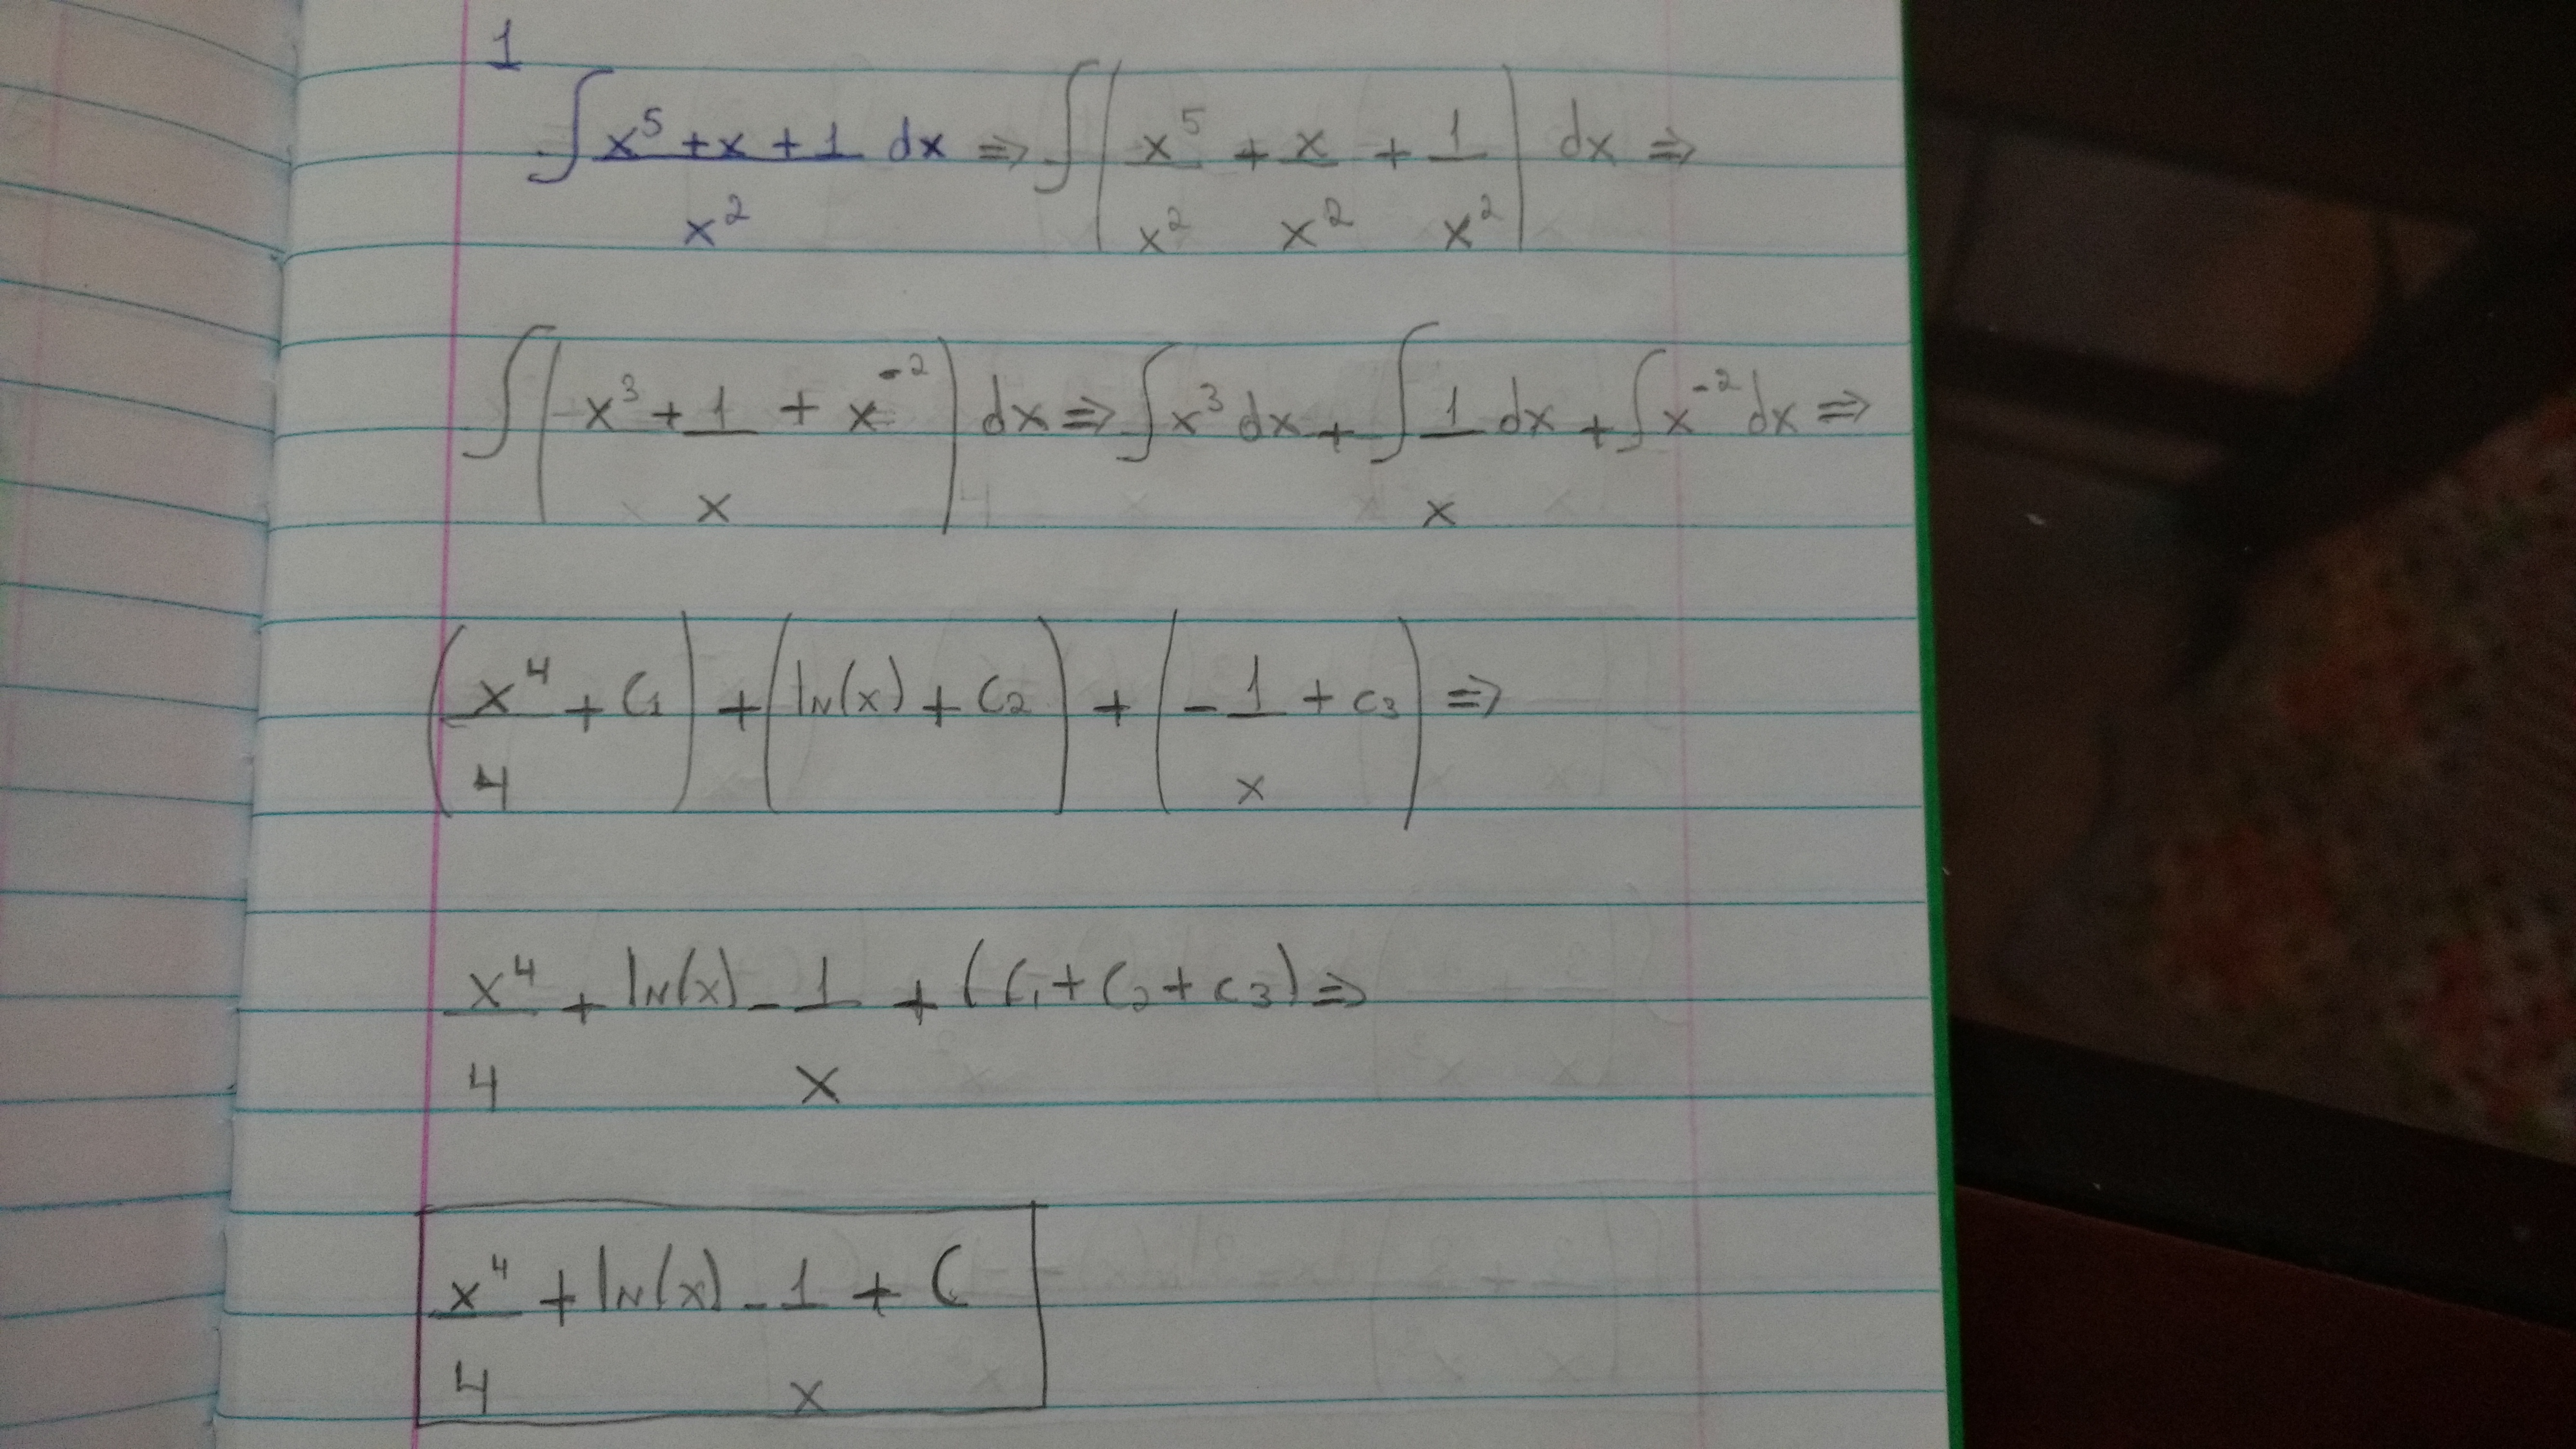
\includegraphics[width=0.9\textwidth]{1}
   \end{figure} \\
\begin{description}
  \item[Sexo:] Qualitativa Nominal
  \item[Peso:] Quantitativa Contínua
  \item[Tipo de Tratamento:] Qualitativa Nominal
  \item[Número de Convulsões:] Quantitativa Discreta
  \item[Classificação da Doença:] Qualitativa Ordinal \\\\
\end{description}
\item Elabore os gráficos solicitados utilizando a tabela de custos de produção Apresentada abaixo:\\
   \begin{figure}[h!]
   \centering
   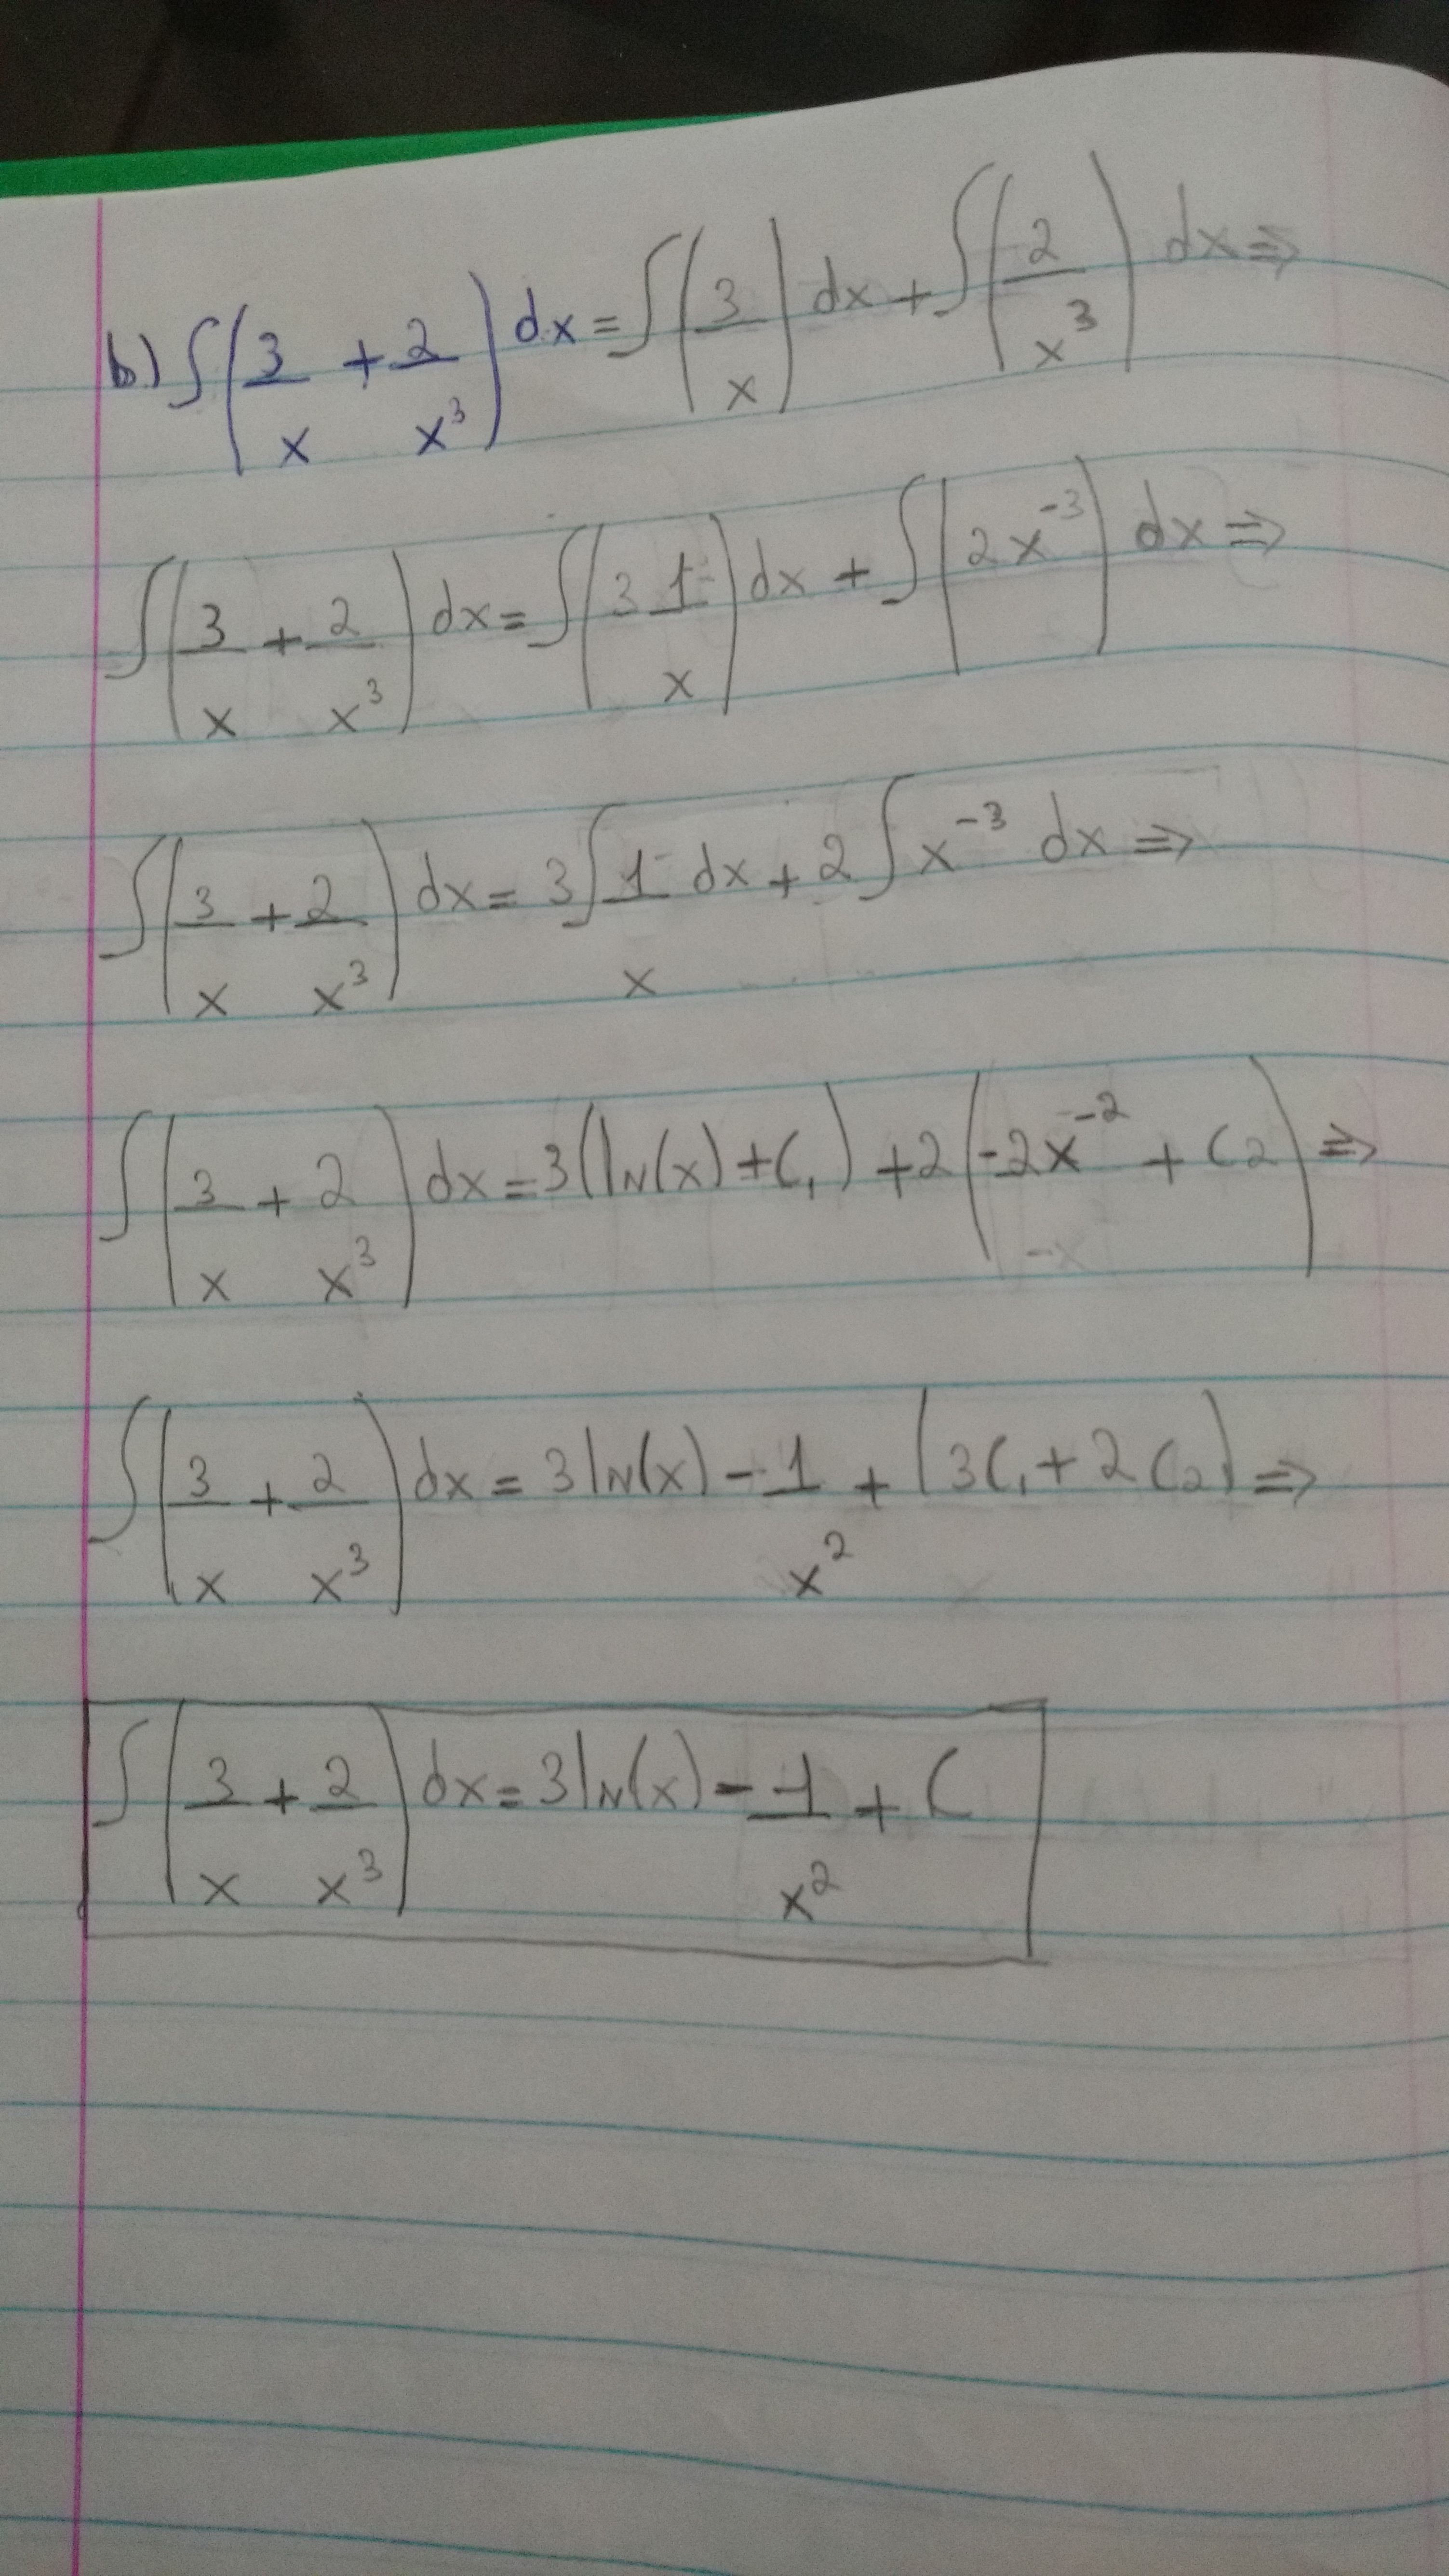
\includegraphics[width=0.9\textwidth]{2}
   \end{figure} \\
\newpage

\begin{enumerate}
  \item Gráfico de colunas contendo custo X frequência simples absoluta.
   \begin{figure}[h!]
   \centering
   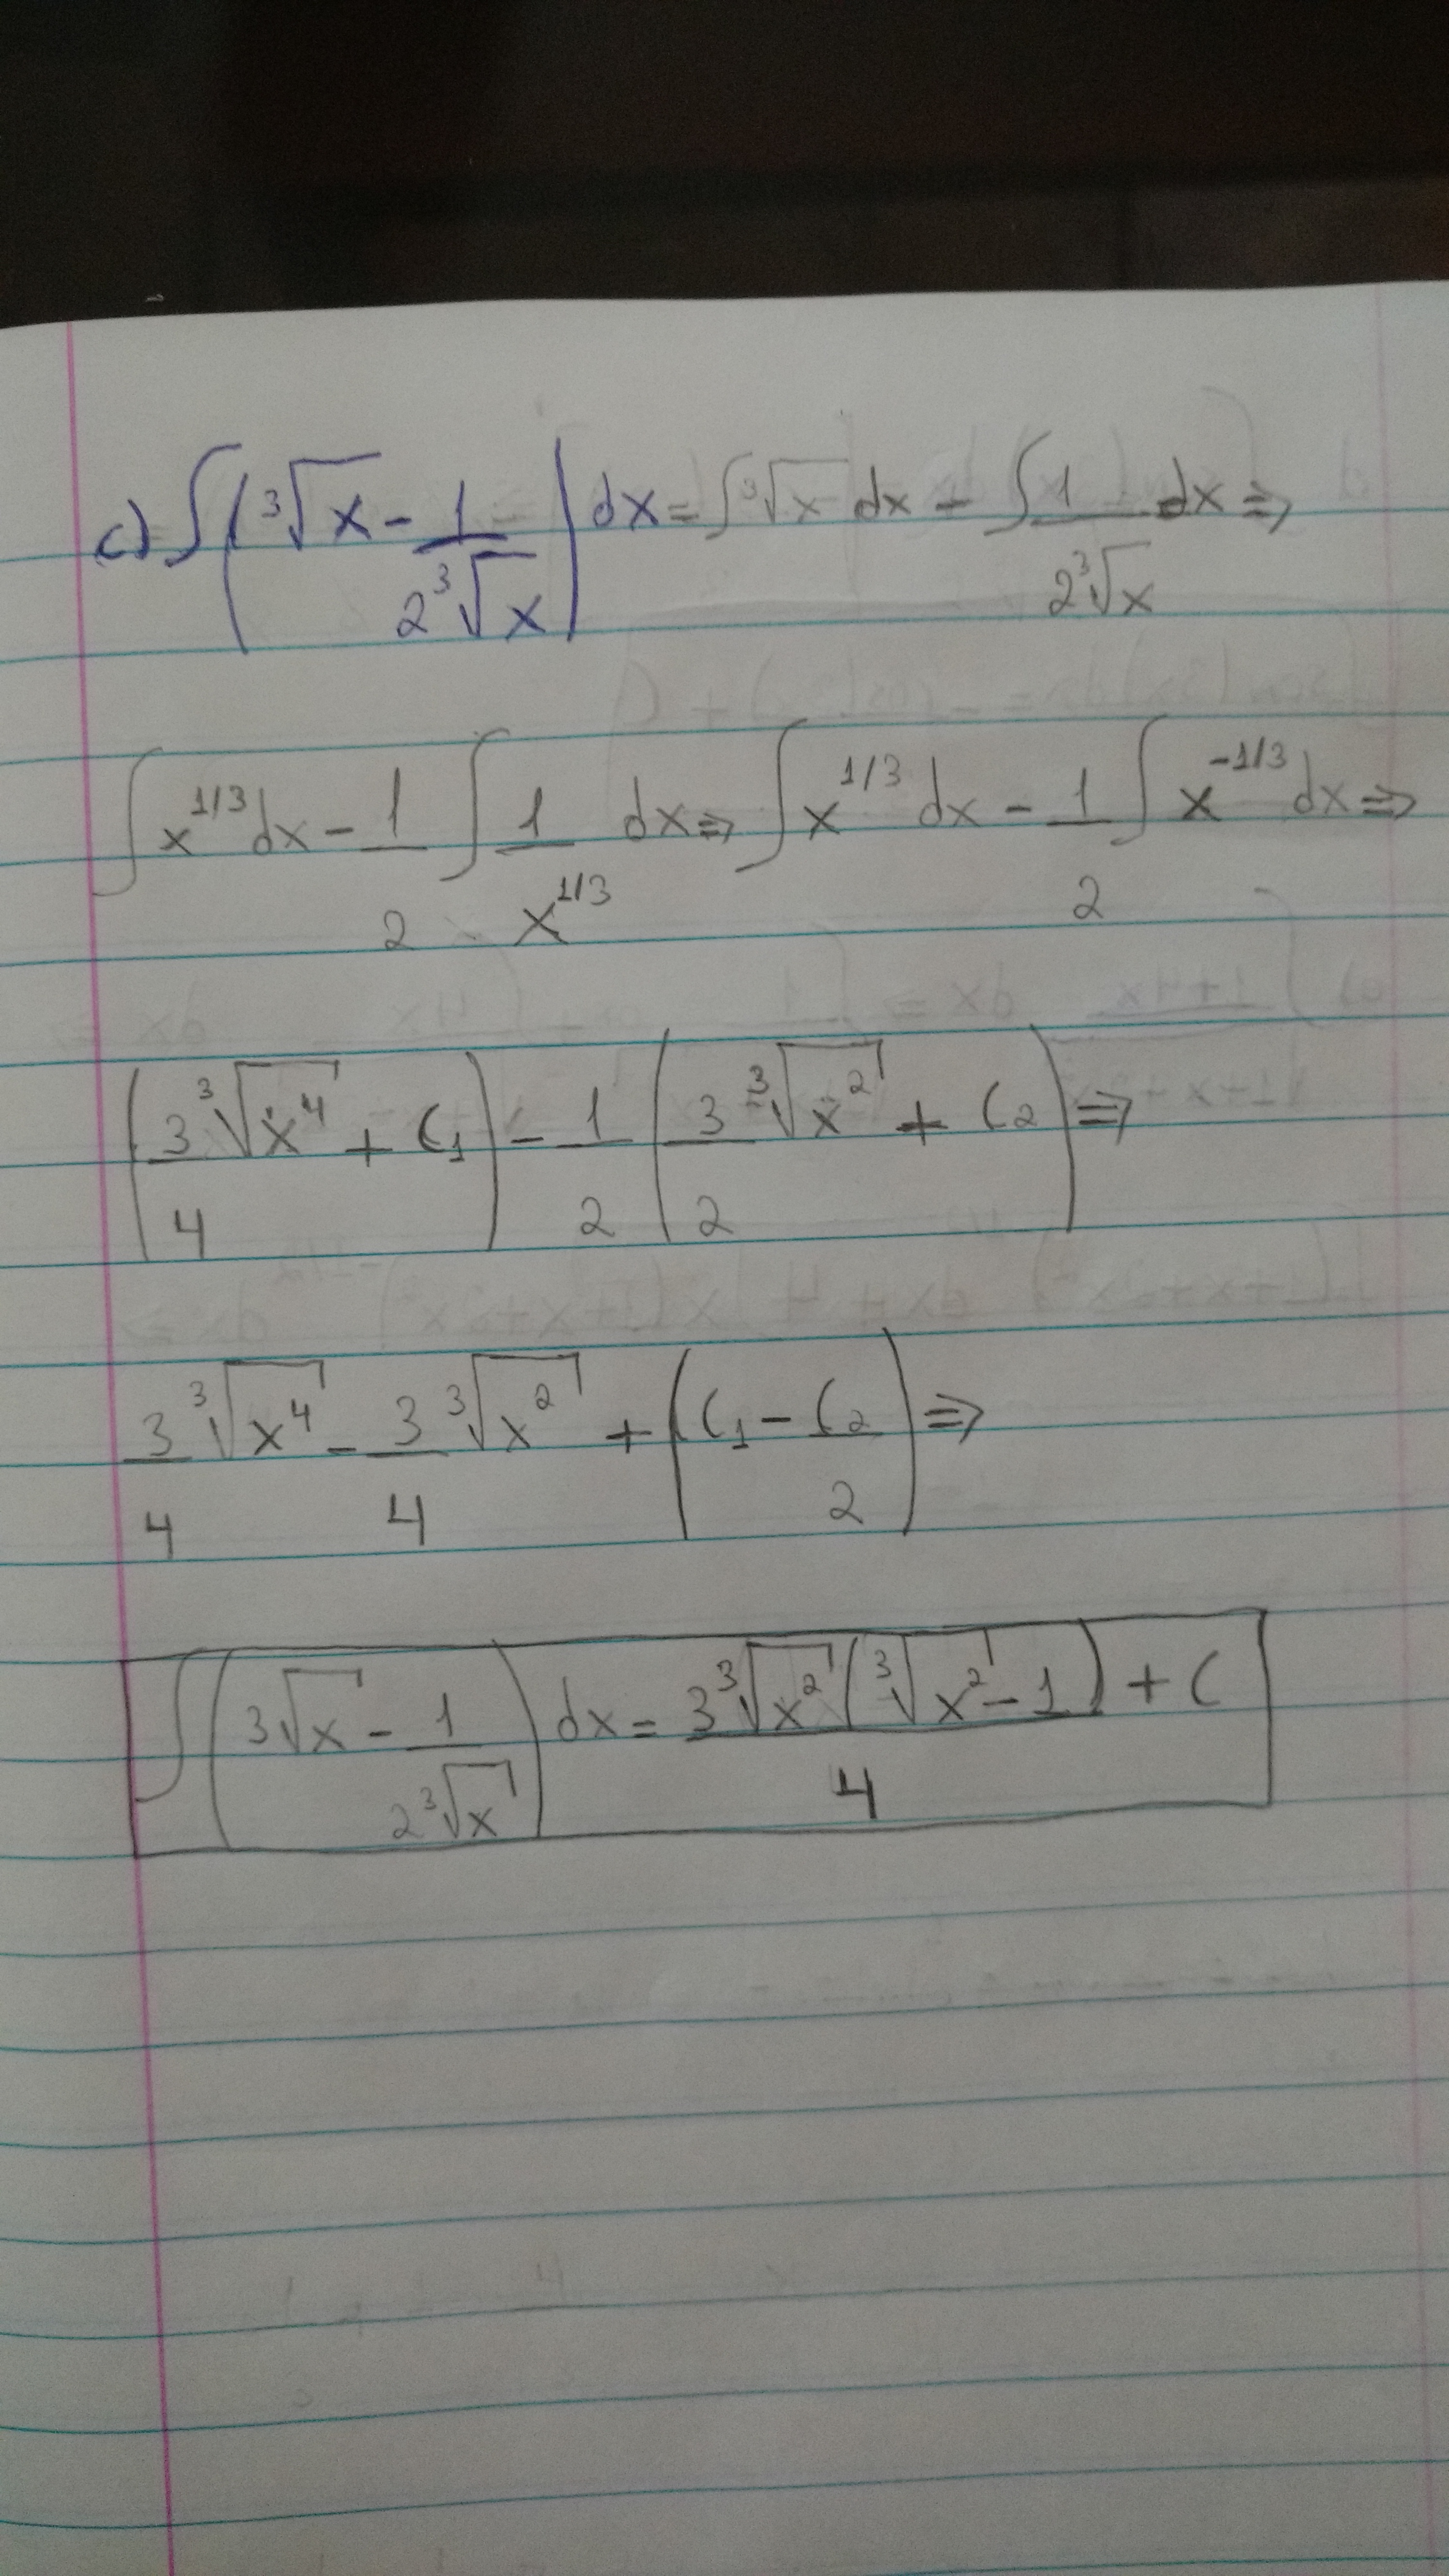
\includegraphics[width=0.9\textwidth]{3}
   \end{figure} \\

\newpage

 \item Gráfico de barras contendo custo X frequência simples relativa.
   \begin{figure}[h!]
   \centering
   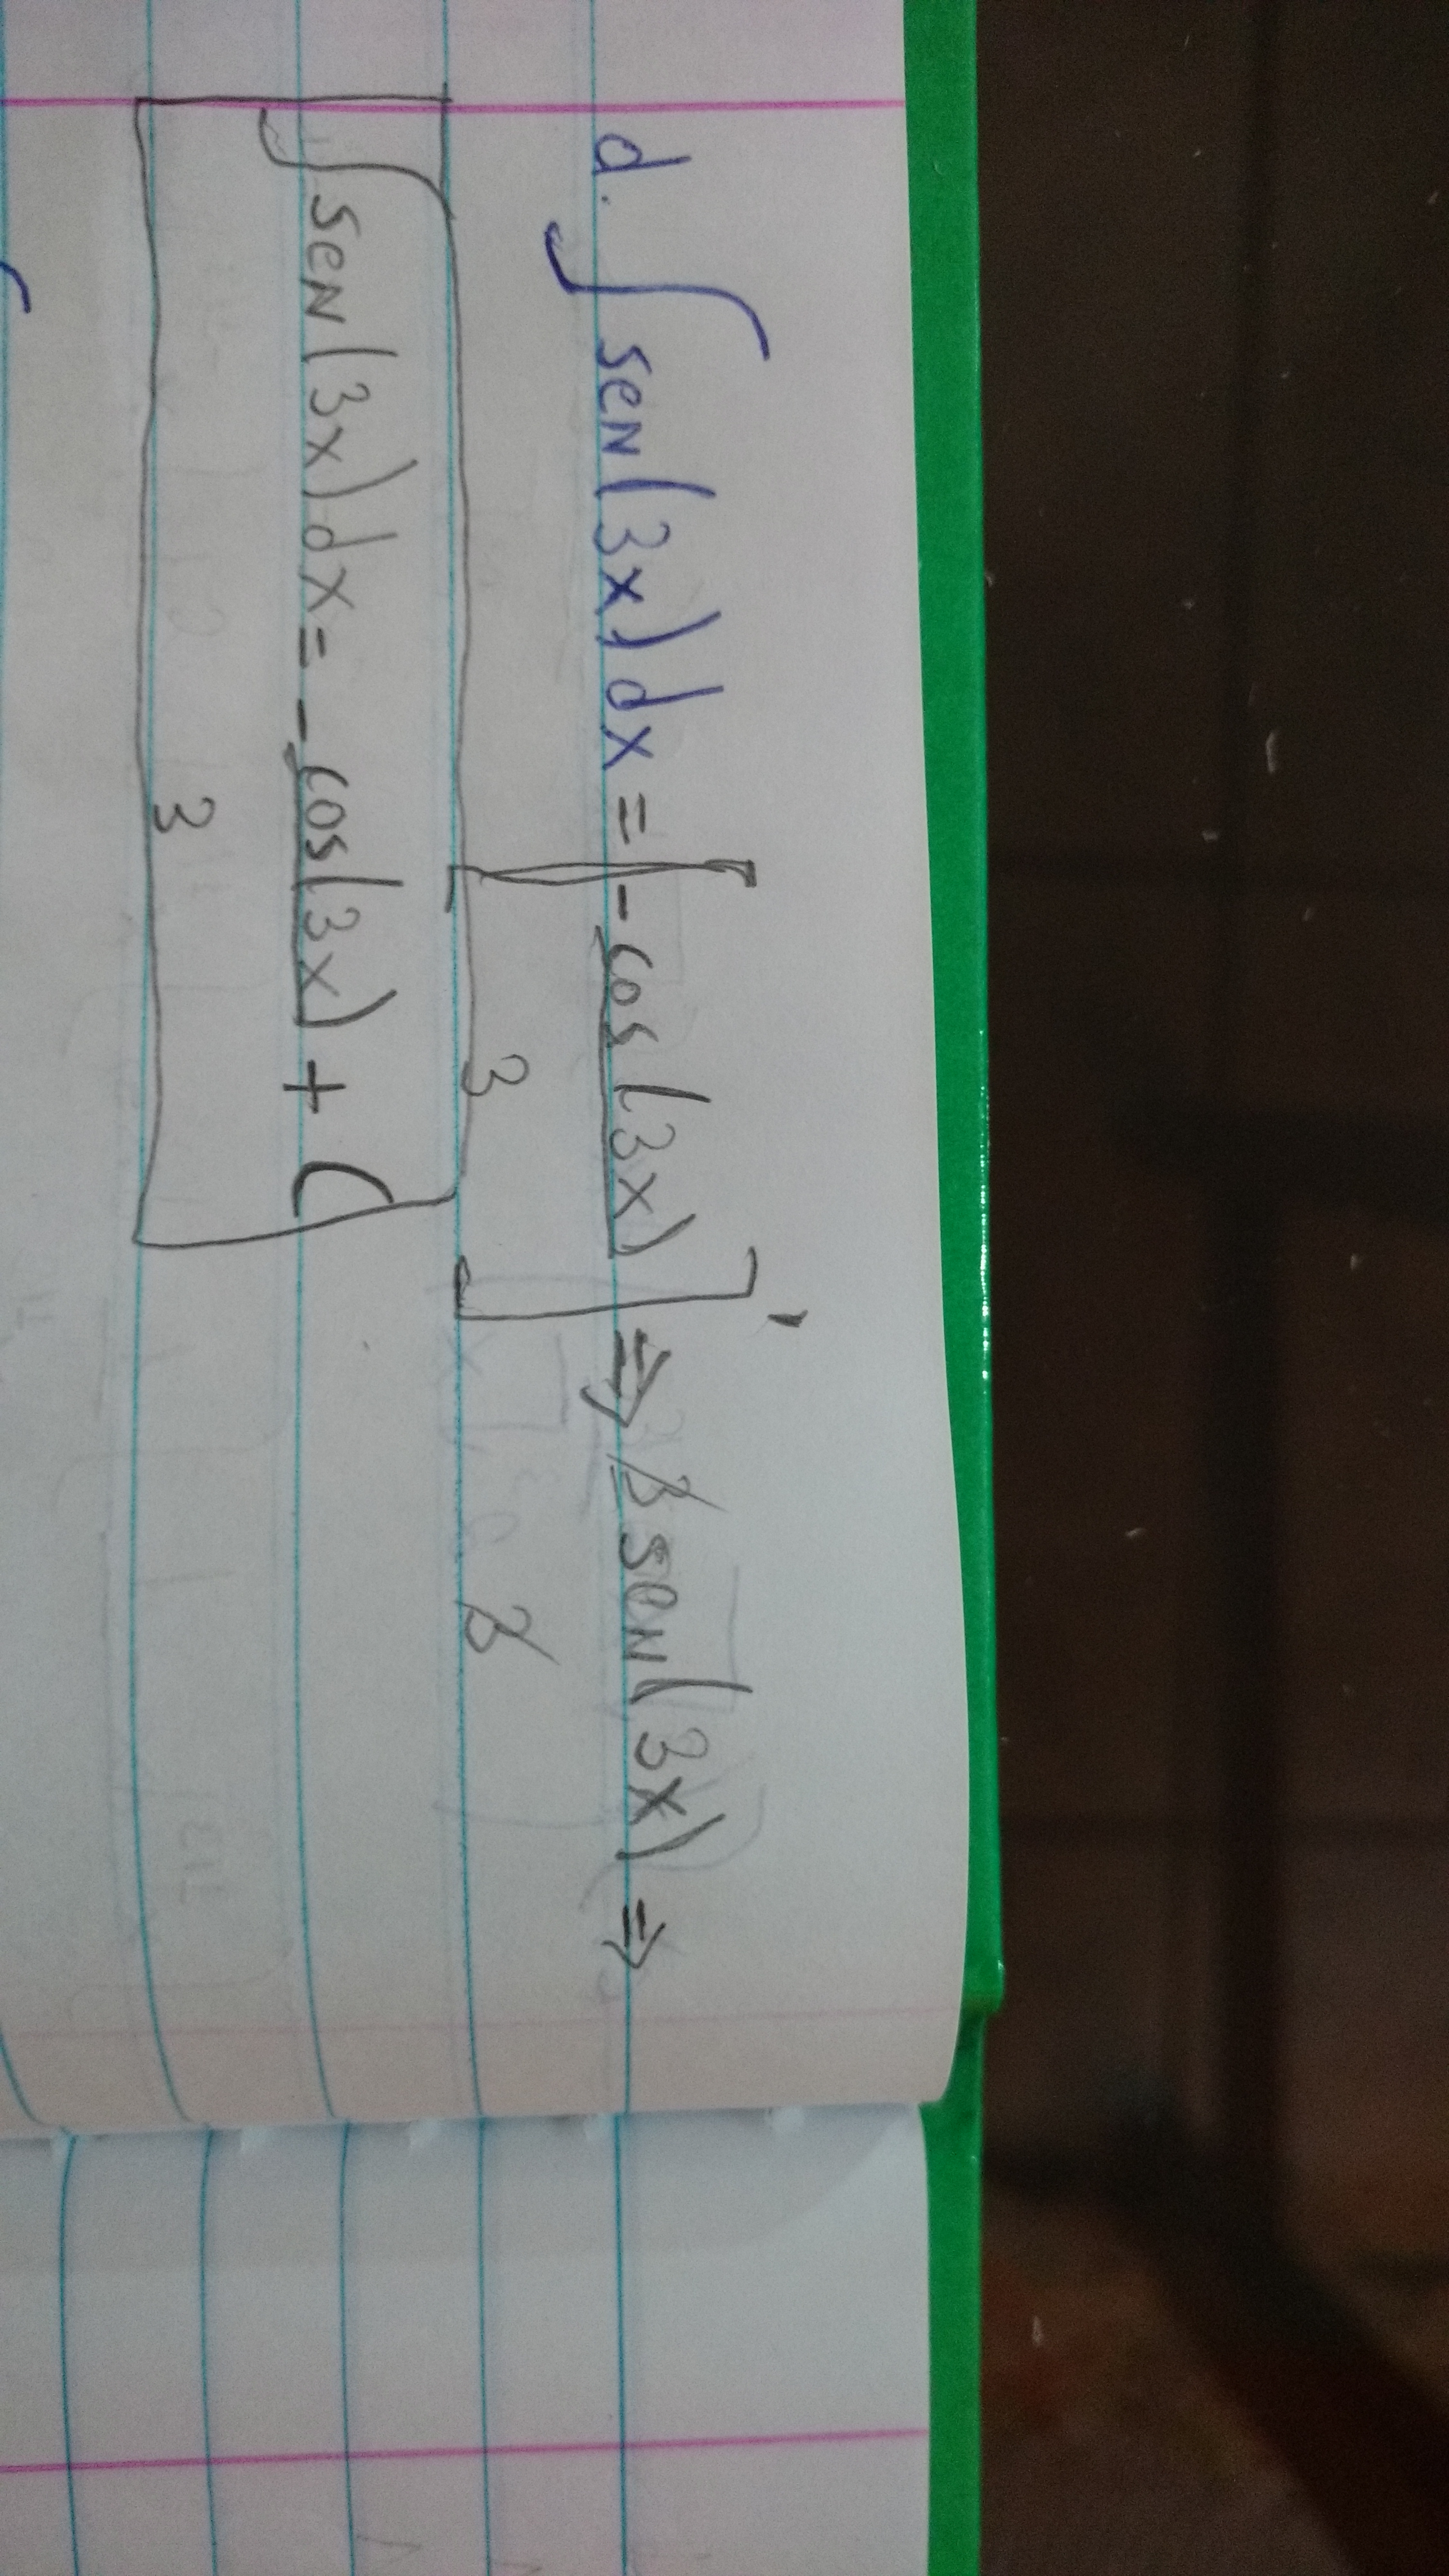
\includegraphics[width=0.9\textwidth]{4}
   \end{figure} \\

\newpage
   
 \item Gráfico de linhas contendo custo X frequência simples absoluta.
   \begin{figure}[h!]
   \centering
   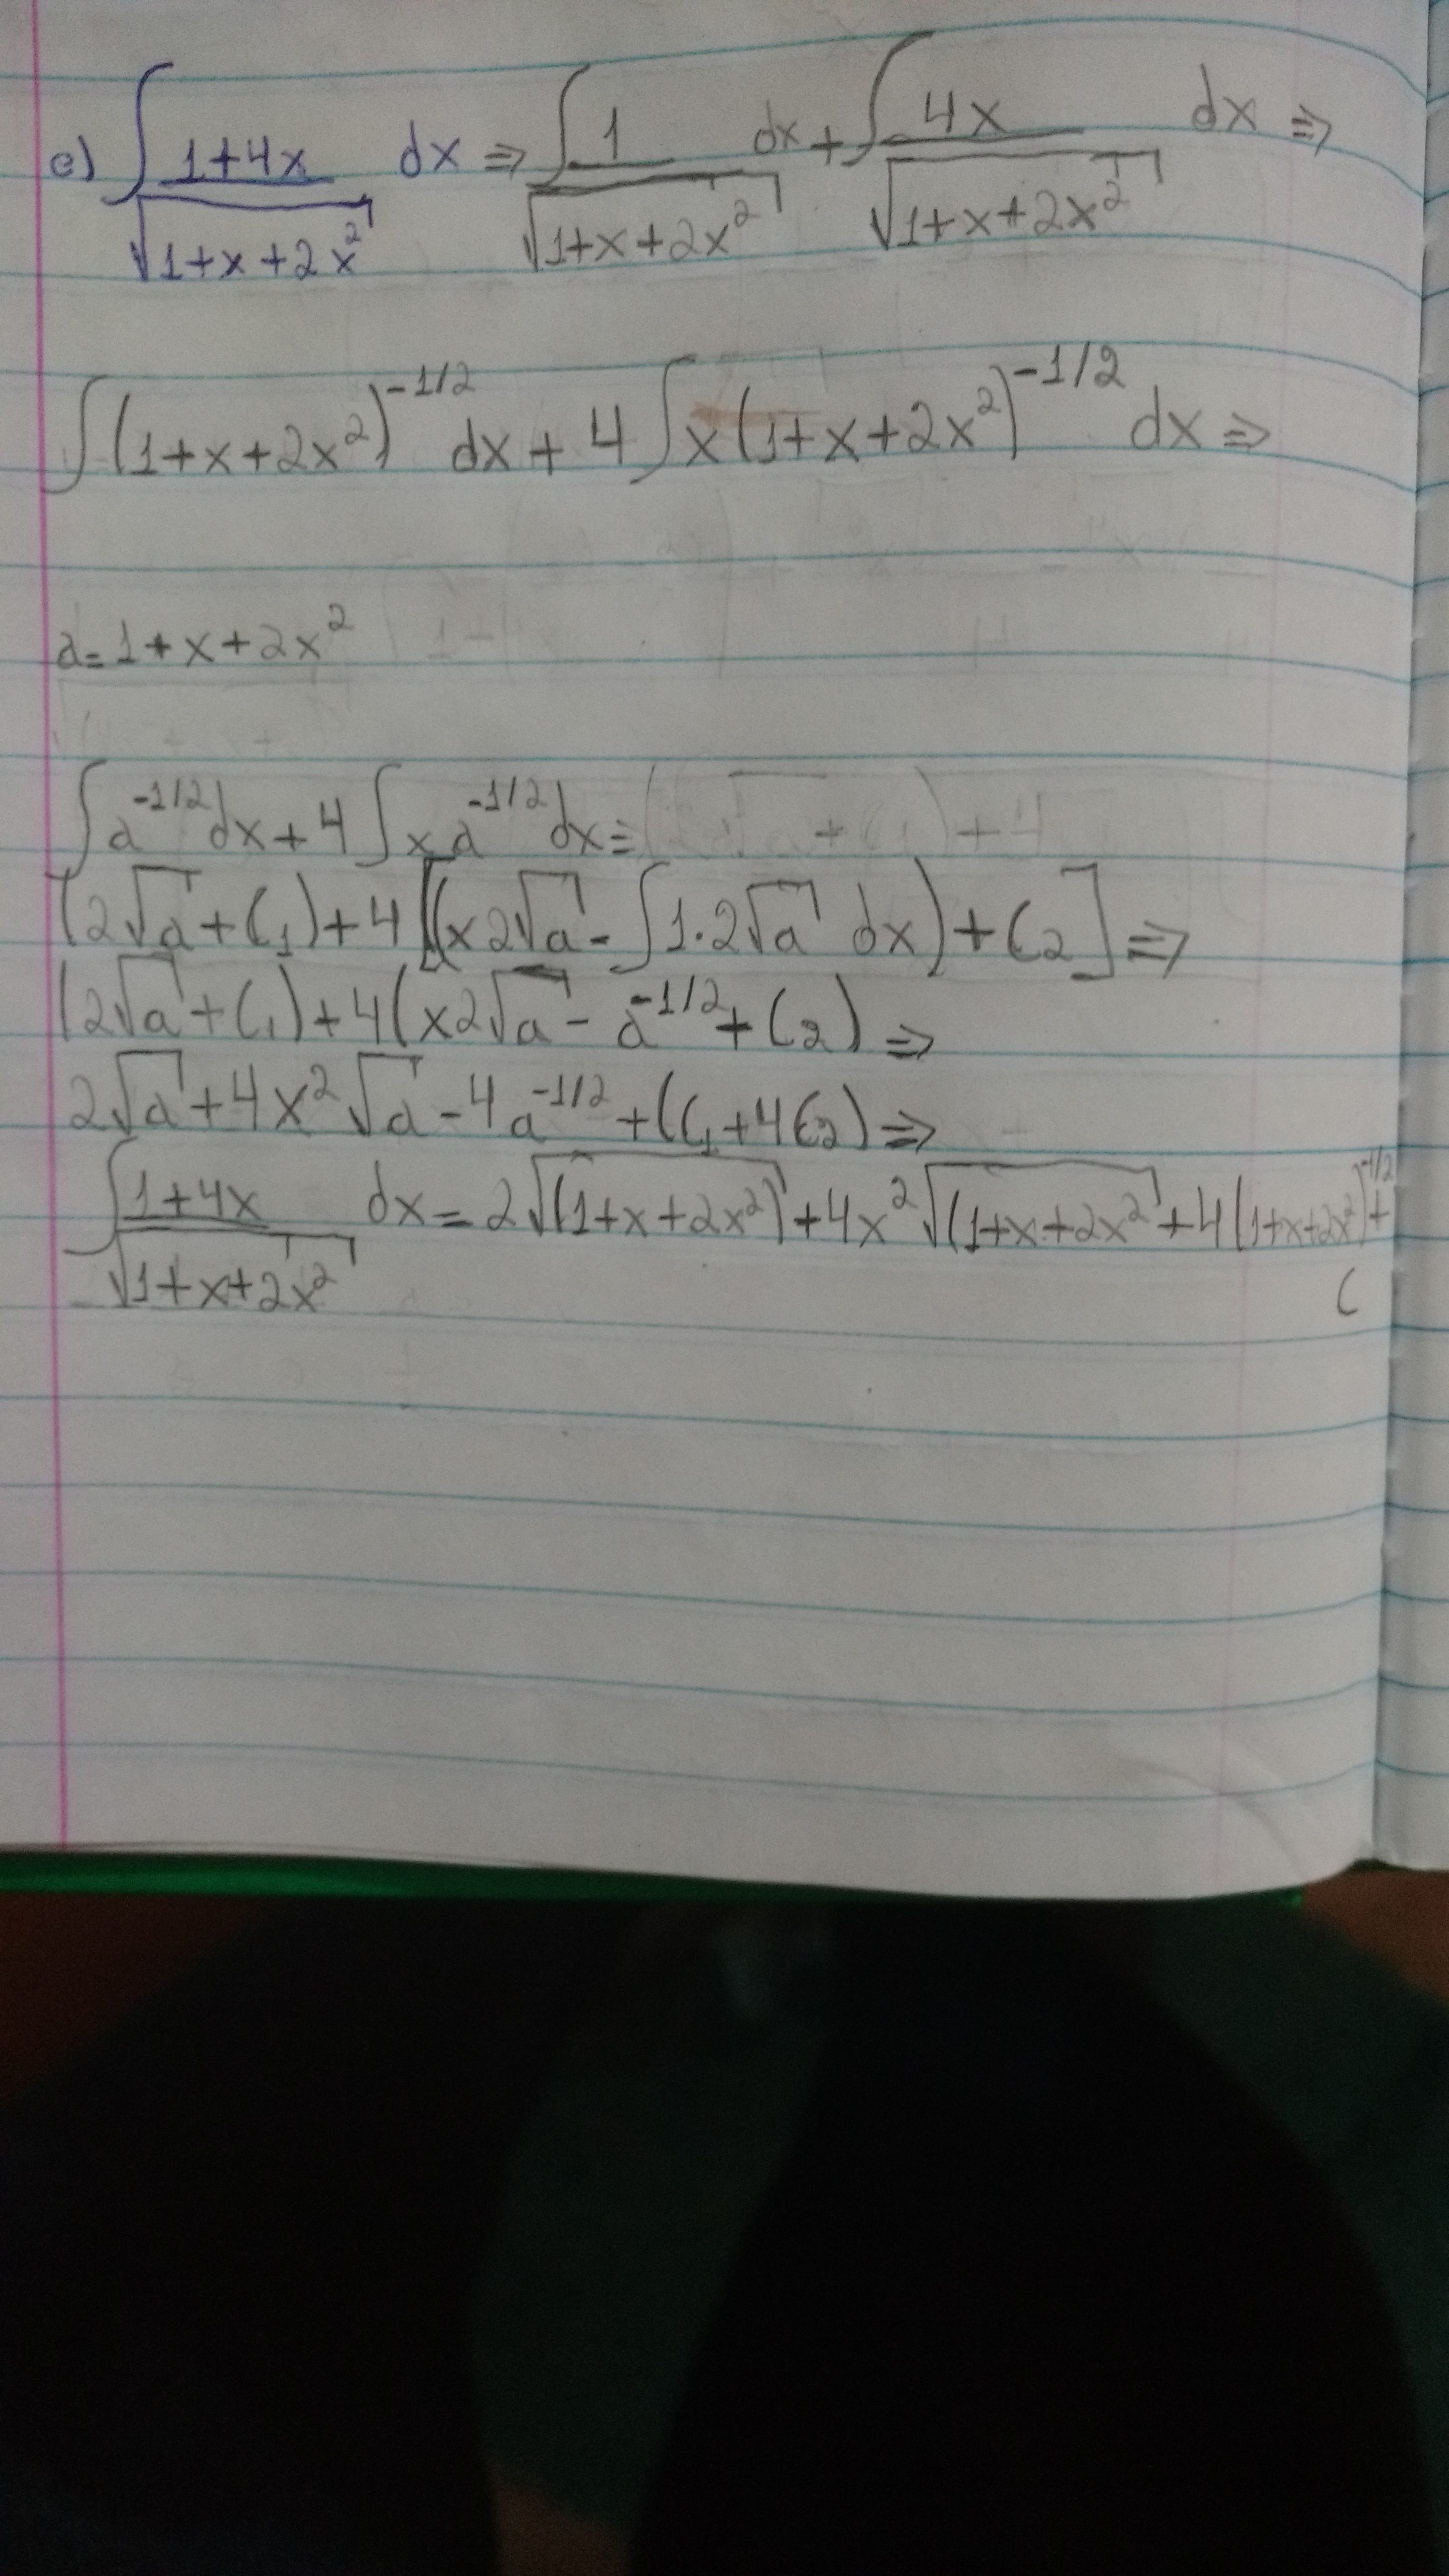
\includegraphics[width=0.9\textwidth]{5}
   \end{figure} \\

\newpage
   
 \item Gráfico de setores contendo custo X frequência simples relativa.
   \begin{figure}[h!]
   \centering
   \includegraphics[width=0.9\textwidth]{6}
   \end{figure} \\
   
\end{enumerate}    
\end{enumerate}  
\end{document}
